\section{Experimental Results}
\label{sec:experimental_results}
    %\TODO{intro. (cf \url{http://frncsrss.github.io/papers/rousseau-ecir2015.pdf})}
    This section presents and analyses the results of our experiments.
    For each document of each dataset, we compare the keyphrases outputed by each method to the reference keyphrases of the document.
    From the comparisons, we compute the macro-averaged precision (P), recall (R) and f1-score (F) per dataset and per method.
        
    \subsection{Macro-averages results}
    \label{subsec:macro_averages_results}
        Table~\ref{tab:comparison_results} presents the macro-averaged precision, recall and f1-score in percentage when 10 keyphrases are extracted/assigned for each dataset by TopicRank, KEA++, TopicCo\-Rank$_{\textit{extr}}$, Topic\-CoRank$_{\textit{assign}}$ and TopicCoRank.
        %
        First, we observe that the assignment baseline KEA++ mostly achieves the lowest performance, which is surprising compared to the performance reported by \newcite{medelyan2006kea++}.
        The first reason for this observation is that KEA++ is restricted to thesauri entries while most keyphrases are missing within our documents.
        The second reason is that KEA++ relies on rich thesauri that contain an important amount of semantic relations between the entries, while our (real application) thesauri have a modest amount of semantic relations between the entries.

        Overall, using graph co-ranking significantly outperforms TopicRank and KEA++.
        Comparing TopicRank to TopicCoRank$_\textit{extr}$ shows the positive influence of the domain (controlled keyphrases) on the ranking of the topics.
        TopicCoRank$_\textit{assign}$ outperforms every method, including TopicCoRank$_\textit{extr}$ and TopicCoRank.
        Controlled keyphrases are efficiently ranked and the predominance of missing keyphrases in the dataset leads to a better performance of TopicCoRank$_\textit{assign}$ over TopicCoRank.
        
        \section{Evaluation}
  \begin{frame}{Evaluation}
    \framesubtitle{Datasets}

    \begin{itemize}
      \item{Inspec contains 500 abstracts of journal papers ({\small\textsc{En}})}
      \begin{itemize}
        \setbeamertemplate{itemize items}[triangle]
        \item{9.8 keyphrases/document}
        \item{21.8\% of missing keyphrases}
      \end{itemize}
    \item{SemEval contains 100 scientific papers ({\small\textsc{En}})}
      \begin{itemize}
        \setbeamertemplate{itemize items}[triangle]
        \item{14.7 keyphrases/document}
        \item{19.3\% of missing keyphrases}
      \end{itemize}
      \item{WikiNews contains 100 news articles ({\small\textsc{Fr}})}
      \begin{itemize}
        \setbeamertemplate{itemize items}[triangle]
        \item{9.6 keyphrases/document}
        \item{4.4\% of missing keyphrases}
      \end{itemize}
      \item{DEFT contains 93 scientific papers ({\small\textsc{Fr}})}
      \begin{itemize}
        \setbeamertemplate{itemize items}[triangle]
        \item{5.2 keyphrases/document}
        \item{18.2\% of missing keyphrases}
      \end{itemize}
    \end{itemize}
  \end{frame}

  \begin{frame}{Evaluation}
    \framesubtitle{Evaluation measures}

    \begin{itemize}
      \item{Cut-off at 10 keyphrases}
      \item{F-score $\Rightarrow$ compromise between precision and recall}
    \end{itemize}

    \begin{center}
      $\text{f-score} = (1 + \beta^2) \times \frac{\text{precision} \times \text{recall}}{(\beta^2 \times precision) + recall}$,
      $\beta = 1$
    \end{center}
  \end{frame}

  \begin{frame}{Evaluation}
    \framesubtitle{Baselines}

    \begin{itemize}
      \item{TF-IDF weighting}
      \begin{itemize}
        \setbeamertemplate{itemize items}[triangle]
        \item{Best keyphrases contain words with hight TF-IDF}
      \end{itemize}
      \item{TextRank}
      \begin{itemize}
        \setbeamertemplate{itemize items}[triangle]
        \item{Word co-occurrence graph with a window of 2}
        \item{PageRank scoring/ranking}
        \item{Keyphrase generation based on keywords}
      \end{itemize}
      \item{SingleRank}
      \begin{itemize}
        \setbeamertemplate{itemize items}[triangle]
        \item{Word co-occurrence graph with a window of 10}
        \item{PageRank scoring/ranking}
        \item{Candidate keyphrases scored/ranked by the sum of their words' PageRank score}
      \end{itemize}
    \end{itemize}

    Redundant keyphrases are removed from the output.
  \end{frame}

  \begin{frame}{Evaluation}
    \framesubtitle{Main results}
    
    \begin{center}
      \begin{tabular}{rcccc}
        \toprule
        Methods & Inspec & SemEval & WikiNews & DEFT\\
        \midrule
        TF-IDF & 33.4 & 10.5 & 34.3 & 13.2\\
        TextRank & 12.7 & $~~$5.6 & $~~$8.6 & $~~$5.7\\
        SingleRank & \cellcolor{pink}{35.2} & $~~$3.7 & 19.7 & $~~$5.9\\
        TopicRank & 27.9 & \cellcolor{pink}{12.1} & \cellcolor{pink}{35.6} & \cellcolor{pink}{15.1}\\
        \bottomrule
      \end{tabular}
    \end{center}
  \end{frame}

  \begin{frame}{Evaluation}
    \framesubtitle{Contributions evaluation}
    
    \begin{center}
      \begin{tabular}{rcccc}
        \toprule
        Methods & Inspec & SemEval & WikiNews & DEFT\\
        \midrule
        SingleRank & 35.2 & $~~$3.7 & 19.7 & $~~$5.9\\
        +phrases & 22.1 & $~~$8.0 & 28.9 & 13.5\\
        +topics & 26.8 & 11.9 & 31.4 & 14.8\\
        +complete &  \cellcolor{pink}{35.5} & $~~$4.4 & 20.3 & $~~$5.8\\
        TopicRank & 27.9 & \cellcolor{pink}{12.1} & \cellcolor{pink}{35.6} & \cellcolor{pink}{15.1}\\
        \bottomrule
      \end{tabular}
    \end{center}
  \end{frame}

  \begin{frame}{Evaluation}
    \framesubtitle{Keyphrase selection evaluation}
    
    \begin{center}
      \resizebox{\linewidth}{!}{
        \begin{tabular}{rcccc}
          \toprule
          Keyphrase selection & Inspec & SemEval & WikiNews & DEFT\\
          \midrule
          \rowcolor{cyan!33} First position & 27.9 & 12.1 & 35.6 & 15.1\\
          Frequency & 26.8 & $~~$1.4 & 26.2 & $~~$2.5\\
          Centroid &  24.7 & $~~$1.5 & 28.5 & $~~$3.4\\
          \rowcolor{pink} Upper bound & 35.6 & 30.3 & 42.9 & 19.3\\
          \bottomrule
        \end{tabular}
      }
    \end{center}
  \end{frame}


  
    \subsection{Precision/recall curves}
    \label{subsec:precision_recall_curves}
        Additionally, we follow \newcite{hassan2010conundrums} and analyse the precision-recall curves of TopicRank, KEA++ and TopicCoRank.
        To generate the curves, we vary the number of evaluated keyphrases (cut-off) from 1 to the total number of extracted/assigned key\-phrases and compute the precision and recall for each cut-off.
        Such representation gives a good appreciation of the advantage of a method compared to others, especially if the other methods achieve performances in the \textit{Area Under the Curve} (AUC).
        
         \begin{figure}[htb!]
            \centering
            \subfigure[Linguistics]{
                \begin{tikzpicture}[scale=.7]
                    \pgfkeys{/pgf/number format/.cd, fixed}
                    \begin{axis}[x=0.0050692\linewidth,
                                 xtick={0, 10, 20, ..., 100},
                                 xmin=0,
                                 xmax=60,
                                 xlabel=recall (\%),
                                 x label style={yshift=.34em},
                                 y=0.0050692\linewidth,
                                 ytick={0, 10, 20, ..., 100},
                                 ymin=0,
                                 ymax=60,
                                 ylabel=precision (\%),
                                 y label style={yshift=-.5em}]
                        \addplot [cyan, mark=+] file {input/data/linguistique_topicrank.csv};
                        \addplot [magenta, mark=o] file {input/data/linguistique_kea_pp.csv};
                        \addplot [blue, mark=x] file {input/data/linguistique_topiccorank.csv};
                        \addplot [dotted, domain=30:60] {(50 * x) / ((2 * x) - 50)};
                        \addplot [dotted, domain=30:60] {(40 * x) / ((2 * x) - 40)};
                        \addplot [dotted, domain=20:60] {(30 * x) / ((2 * x) - 30)};
                        \addplot [dotted, domain=10:60] {(20 * x) / ((2 * x) - 20)};
                        \addplot [dotted, domain=5:60] {(10 * x) / ((2 * x) - 10)};
                        \legend{TopicRank, KEA++, TopicCoRank};
                    \end{axis}
                    %\node at (3.8,2.9) [anchor=east] {\scriptsize{F=50.0}};
                    \node at (4.9,2.6) [anchor=east] {\scriptsize{F=40.0}};
                    \node at (4.9,1.8) [anchor=east] {\scriptsize{F=30.0}};
                    \node at (4.9,1.15) [anchor=east] {\scriptsize{F=20.0}};
                    \node at (4.9,0.6) [anchor=east] {\scriptsize{F=10.0}};
                \end{tikzpicture}
            }
            \subfigure[Information Science]{
                \begin{tikzpicture}[scale=.7]
                    \pgfkeys{/pgf/number format/.cd, fixed}
                    \begin{axis}[x=0.0050692\linewidth,
                                 xtick={0, 10, 20, ..., 100},
                                 xmin=0,
                                 xmax=60,
                                 xlabel=recall (\%),
                                 x label style={yshift=.34em},
                                 y=0.0050692\linewidth,
                                 ytick={0, 10, 20, ..., 100},
                                 ymin=0,
                                 ymax=60,
                                 ylabel=precision (\%),
                                 y label style={yshift=-.5em}]
                        \addplot [cyan, mark=+] file {input/data/sciences_de_l_information_topicrank.csv};
                        \addplot [magenta, mark=o] file {input/data/sciences_de_l_information_kea_pp.csv};
                        \addplot [blue, mark=x] file {input/data/sciences_de_l_information_topiccorank.csv};
                        \addplot [dotted, domain=30:60] {(50 * x) / ((2 * x) - 50)};
                        \addplot [dotted, domain=30:60] {(40 * x) / ((2 * x) - 40)};
                        \addplot [dotted, domain=20:60] {(30 * x) / ((2 * x) - 30)};
                        \addplot [dotted, domain=10:60] {(20 * x) / ((2 * x) - 20)};
                        \addplot [dotted, domain=5:60] {(10 * x) / ((2 * x) - 10)};
                    \end{axis}
                    \node at (4.9,3.7) [anchor=east] {\scriptsize{F=50.0}};
                    \node at (4.9,2.6) [anchor=east] {\scriptsize{F=40.0}};
                    \node at (4.9,1.8) [anchor=east] {\scriptsize{F=30.0}};
                    \node at (4.9,1.15) [anchor=east] {\scriptsize{F=20.0}};
                    \node at (4.9,0.6) [anchor=east] {\scriptsize{F=10.0}};
                \end{tikzpicture}
            }
            \subfigure[Archaeology]{
                \begin{tikzpicture}[scale=.7]
                    \pgfkeys{/pgf/number format/.cd, fixed}
                    \begin{axis}[x=0.0050692\linewidth,
                                 xtick={0, 10, 20, ..., 100},
                                 xmin=0,
                                 xmax=60,
                                 xlabel=recall (\%),
                                 x label style={yshift=.34em},
                                 y=0.0050692\linewidth,
                                 ytick={0, 10, 20, ..., 100},
                                 ymin=0,
                                 ymax=60,
                                 ylabel=precision (\%),
                                 y label style={yshift=-.5em},
                                 legend style={font=\footnotesize}]
                        \addplot [cyan, mark=+] file {input/data/archeologie_topicrank.csv};
                        \addplot [magenta, mark=o] file {input/data/archeologie_kea_pp.csv};
                        \addplot [blue, mark=x] file {input/data/archeologie_topiccorank.csv};
                        \addplot [dotted, domain=30:60] {(50 * x) / ((2 * x) - 50)};
                        \addplot [dotted, domain=30:60] {(40 * x) / ((2 * x) - 40)};
                        \addplot [dotted, domain=20:60] {(30 * x) / ((2 * x) - 30)};
                        \addplot [dotted, domain=10:60] {(20 * x) / ((2 * x) - 20)};
                        \addplot [dotted, domain=5:60] {(10 * x) / ((2 * x) - 10)};
                    \end{axis}
                    \node at (4.9,3.7) [anchor=east] {\scriptsize{F=50.0}};
                    \node at (4.9,2.6) [anchor=east] {\scriptsize{F=40.0}};
                    \node at (4.9,1.8) [anchor=east] {\scriptsize{F=30.0}};
                    \node at (4.9,1.15) [anchor=east] {\scriptsize{F=20.0}};
                    \node at (4.9,0.6) [anchor=east] {\scriptsize{F=10.0}};
                \end{tikzpicture}
            }
            \caption{
                Precision-recall curves of TopicRank, KEA++ and TopicCoRank for each dataset
                \label{fig:pr_curves}
            }
        \end{figure}

        Figure~\ref{fig:pr_curves} shows the precision/recall curves of TopicRank, KEA++ and TopicCoRank on each dataset.
        The final recall for the methods does not reach 100\% because the candidate selection method does not provide keyphrases that do not occur within the document, as well as candidates that do not fit the POS tag pattern \texttt{/(N|A)+/}.
        Also, because TopicRank and TopicCoRank topically cluster keyphrase candidates and output only one candidate per topic, their final recall is lowered every time a wrong keyphrase is chosen over a correct one from the topic.
 
        We observe that the curve for TopicCoRank is systematically above the others, thus showing improvements in the area under the curve and not just in point estimate such as f1-score.
        Also, the final recall of TopicCoRank is much higher than the final recall of TopicRank and KEA++.
       
      
    
    \subsection{Extraction vs. assignment}
    \label{subsec:assignment_vs_extraction}
        As TopicCoRank is the first method for simultaneously extracting and assigning key\-phrases, we perform an additional experiment that shows to which extent extraction and assignment contribute to the final results.
        %Table~\ref{tab:assignment_ratio} shows the percentage of the first ten keyphrases extracted from the topics of the document graph and assigned from the domain graph.
        %TopicCoRank succesfully performs extraction and assignment simultaneously.
        %However, although most reference keyphrases have to be assigned, the ratio of assignment is lower than the ratio of extraction.
        %During the co-ranking, we observe that topics get higher scores than controlled keyphrases and the extraction, therefore, becomes ascendant.
        %\begin{table}[t]
        %    \centering
        %    \begin{tabular}{l|c@{\hspace{1em}}c@{\hspace{1em}}c}
        %        \toprule
        %        & \textbf{Linguistics} & \textbf{Information Science} & \textbf{Archaeology}\\
        %        \hline
        %            Extraction & 56.9\% & 71.0\% & 78.2\%\\
        %            Assignment & 43.1\% & 29.0\% & 21.8\%\\
        %        \bottomrule
        %    \end{tabular}
        %    \caption{Average ratio of assignment performed by TopicCoRank at 10 keyphrases
        %             \label{tab:assignment_ratio}}
        %\end{table}
        %
        To do so, we show the behavior of the extraction and the assignment depending on the influence of the inner recommendation on the ranking for each (test) document of each dataset.
        
        Fig.~\ref{fig:lambda_t_variation} shows the behavior of TopicCoRank$_\textit{extr}$ when $\lambda_t$ varies from 0 to 1.
        When $\lambda_t = 0$, only the domain influences the ranking of the topics.
        Slightly equivalent to KEA++, TopicCoRank$_\textit{extr}$ with $\lambda_t = 0$ mainly extracts keyphrases from topics connected to controlled keyphrases.
        When $\lambda_t = 1$, the domain does not influence the ranking and the performance of TopicCoRank$_\textit{extr}$ is in the range of TopicRank's performance.
        Overall, the performance curve of TopicCoRank$_\textit{extr}$ decreases while $\lambda_t$ increases.
        Thus, the experiment demonstrates that the domain has a positive influence on the keyphrase extraction.
        
        \begin{figure}[htb!]
            \centering
            \subfigure[Linguistics]{
                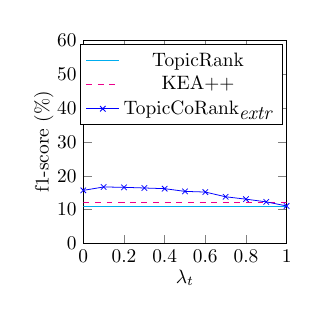
\begin{tikzpicture}[scale=.7]
                    \pgfkeys{/pgf/number format/.cd, fixed}
                    \begin{axis}[x=0.304152\linewidth,
                                 xtick={0, 0.2, 0.4, ..., 1},
                                 xmin=0,
                                 xmax=1,
                                 xlabel=$\lambda_t$,
                                 x label style={yshift=.34em},
                                 y=0.0050692\linewidth,
                                 ytick={0, 10, 20, ..., 100},
                                 ymin=0,
                                 ymax=60,
                                 ylabel=f1-score (\%),
                                 y label style={yshift=-.5em}]
                        \addplot[cyan] coordinates{
                            (0.0, 11)
                            (0.2, 11)
                            (0.3, 11)
                            (0.4, 11)
                            (0.5, 11)
                            (0.6, 11)
                            (0.7, 11)
                            (0.8, 11)
                            (0.9, 11)
                            (1.0, 11)
                        };
                        \addplot[magenta, dashed] coordinates{
                            (0.0, 12)
                            (0.2, 12)
                            (0.3, 12)
                            (0.4, 12)
                            (0.5, 12)
                            (0.6, 12)
                            (0.7, 12)
                            (0.8, 12)
                            (0.9, 12)
                            (1.0, 12)
                        };
                        \addplot[blue, mark=x] coordinates{
                            (0.0, 15.7)
                            (0.1, 16.7)
                            (0.2, 16.6)
                            (0.3, 16.4)
                            (0.4, 16.2)
                            (0.5, 15.4)
                            (0.6, 15.2)
                            (0.7, 13.8)
                            (0.8, 13.1)
                            (0.9, 12.3)
                            (1.0, 11.1)
                        };
                        \legend{TopicRank, KEA++, TopicCoRank$_\textit{extr}$};
                    \end{axis}
                \end{tikzpicture}
            }
            \subfigure[Information Science]{
                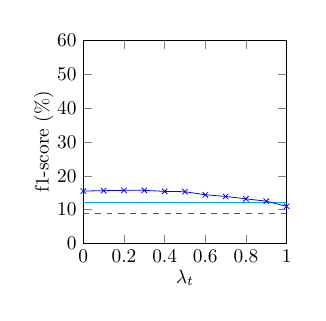
\begin{tikzpicture}[scale=.7]
                    \pgfkeys{/pgf/number format/.cd, fixed}
                    \begin{axis}[x=0.304152\linewidth,
                                 xtick={0, 0.2, 0.4, ..., 1},
                                 xmin=0,
                                 xmax=1,
                                 xlabel=$\lambda_t$,
                                 x label style={yshift=.34em},
                                 y=0.0050692\linewidth,
                                 ytick={0, 10, 20, ..., 100},
                                 ymin=0,
                                 ymax=60,
                                 ylabel=f1-score (\%),
                                 y label style={yshift=-.5em}]
                        \addplot[cyan] coordinates{
                            (0.0, 12)
                            (0.2, 12)
                            (0.3, 12)
                            (0.4, 12)
                            (0.5, 12)
                            (0.6, 12)
                            (0.7, 12)
                            (0.8, 12)
                            (0.9, 12)
                            (1.0, 12)
                        };
                        \addplot[magenta, dashed] coordinates{
                            (0.0, 9)
                            (0.2, 9)
                            (0.3, 9)
                            (0.4, 9)
                            (0.5, 9)
                            (0.6, 9)
                            (0.7, 9)
                            (0.8, 9)
                            (0.9, 9)
                            (1.0, 9)
                        };
                        \addplot[blue, mark=x] coordinates{
                            (0.0, 15.5)
                            (0.1, 15.6)
                            (0.2, 15.7)
                            (0.3, 15.7)
                            (0.4, 15.4)
                            (0.5, 15.3)
                            (0.6, 14.4)
                            (0.7, 13.9)
                            (0.8, 13.2)
                            (0.9, 12.5)
                            (1.0, 11.0)
                        };
                    \end{axis}
                \end{tikzpicture}
            }
            \subfigure[Archaeology]{
                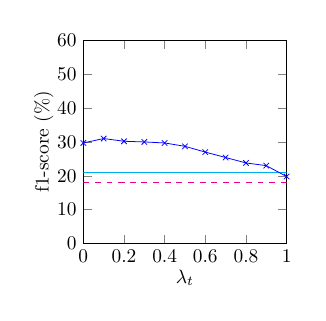
\begin{tikzpicture}[scale=.7]
                    \pgfkeys{/pgf/number format/.cd, fixed}
                    \begin{axis}[x=0.304152\linewidth,
                                 xtick={0, 0.2, 0.4, ..., 1},
                                 xmin=0,
                                 xmax=1,
                                 xlabel=$\lambda_t$,
                                 x label style={yshift=.34em},
                                 y=0.0050692\linewidth,
                                 ytick={0, 10, 20, ..., 100},
                                 ymin=0,
                                 ymax=60,
                                 ylabel=f1-score (\%),
                                 y label style={yshift=-.5em},
                                 legend style={font=\footnotesize}]
                        \addplot[cyan] coordinates{
                            (0.0, 21)
                            (0.2, 21)
                            (0.3, 21)
                            (0.4, 21)
                            (0.5, 21)
                            (0.6, 21)
                            (0.7, 21)
                            (0.8, 21)
                            (0.9, 21)
                            (1.0, 21)
                        };
                        \addplot[magenta, dashed] coordinates{
                            (0.0, 18)
                            (0.2, 18)
                            (0.3, 18)
                            (0.4, 18)
                            (0.5, 18)
                            (0.6, 18)
                            (0.7, 18)
                            (0.8, 18)
                            (0.9, 18)
                            (1.0, 18)
                        };
                        \addplot[blue, mark=x] coordinates{
                            (0.0, 29.7)
                            (0.1, 31.0)
                            (0.2, 30.2)
                            (0.3, 30.0)
                            (0.4, 29.7)
                            (0.5, 28.7)
                            (0.6, 27.0)
                            (0.7, 25.4)
                            (0.8, 23.8)
                            (0.9, 23.0)
                            (1.0, 19.8)
                        };
                    \end{axis}
                \end{tikzpicture}
            }
            \caption{
                Behavior of TopicCoRank$_\textit{extr}$ depending on $\lambda_t$ ($\lambda_k = 0.5$)
                \label{fig:lambda_t_variation}
            }
        \end{figure}
        
        %\begin{figure}[t]
        %    \centering
        %    \subfigure[TopicCoRank$_\textit{extr}$~($\lambda_k$~$=$~$0.5$)\label{subfig:topiccorank_extr}]{
        %        \begin{tikzpicture}[scale=.6]
        %            \pgfkeys{/pgf/number format/.cd, fixed}
        %            \begin{axis}[x=0.5\linewidth,
        %                         xtick={0, 0.2, ..., 1.0},
        %                         xmin=0.0,
        %                         xmax=1.0,
        %                         xlabel=$\lambda_t$,
        %                         x label style={yshift=.34em},
        %                         y=0.0083375\textheight,
        %                         ytick={0, 4, ..., 100},
        %                         ymin=4,
        %                         ymax=44,
        %                         ylabel=f1-score (\%),
        %                         y label style={yshift=-1.1em}]
        %                \addplot[cyan, mark=+] coordinates{
        %                    (0.0, 15.7)
        %                    (0.1, 16.7)
        %                    (0.2, 16.6)
        %                    (0.3, 16.4)
        %                    (0.4, 16.2)
        %                    (0.5, 15.4)
        %                    (0.6, 15.2)
        %                    (0.7, 13.8)
        %                    (0.8, 13.1)
        %                    (0.9, 12.3)
        %                    (1.0, 11.1)
        %                };
        %                \addplot[magenta, mark=o] coordinates{
        %                    (0.0, 15.5)
        %                    (0.1, 15.6)
        %                    (0.2, 15.7)
        %                    (0.3, 15.7)
        %                    (0.4, 15.4)
        %                    (0.5, 15.3)
        %                    (0.6, 14.4)
        %                    (0.7, 13.9)
        %                    (0.8, 13.2)
        %                    (0.9, 12.5)
        %                    (1.0, 11.0)
        %                };
        %                \addplot[black!75, mark=x] coordinates{
        %                    (0.0, 29.7)
        %                    (0.1, 31.0)
        %                    (0.2, 30.2)
        %                    (0.3, 30.0)
        %                    (0.4, 29.7)
        %                    (0.5, 28.7)
        %                    (0.6, 27.0)
        %                    (0.7, 25.4)
        %                    (0.8, 23.8)
        %                    (0.9, 23.0)
        %                    (1.0, 19.8)
        %                };
        %                \legend{Linguistics, Information Science, Archaeology};
        %            \end{axis}
        %        \end{tikzpicture}
        %    }
        %    \hspace{1em}
        %    \subfigure[TopicCoRank$_\textit{assign}$~($\lambda_t$~$=$~$0.1$)\label{subfig:topiccorank_assign}]{
        %        \begin{tikzpicture}[scale=.6]
        %            \pgfkeys{/pgf/number format/.cd, fixed}
        %            \begin{axis}[x=0.5\linewidth,
        %                         xtick={0, 0.2, ..., 1.0},
        %                         xmin=0.0,
        %                         xmax=1.0,
        %                         xlabel=$\lambda_k$,
        %                         x label style={yshift=.34em},
        %                         y=0.0083375\textheight,
        %                         ytick={0, 4, ..., 100},
        %                         ymin=4,
        %                         ymax=44,
        %                         ylabel=f1-score (\%),
        %                         y label style={yshift=-1.1em}]
        %                \addplot[cyan, mark=+] coordinates{
        %                    (0.0, 21.0)
        %                    (0.2, 24.7)
        %                    (0.3, 25.4)
        %                    (0.4, 25.7)
        %                    (0.5, 27.2)
        %                    (0.6, 24.9)
        %                    (0.7, 18.0)
        %                    (0.8, 17.0)
        %                    (0.9, 16.6)
        %                    (1.0, 16.4)
        %                };
        %                \addplot[magenta, mark=o] coordinates{
        %                    (0.0, 17.6)
        %                    (0.1, 18.4)
        %                    (0.2, 18.3)
        %                    (0.3, 18.6)
        %                    (0.4, 19.2)
        %                    (0.5, 19.5)
        %                    (0.6, 19.4)
        %                    (0.7, 11.8)
        %                    (0.8, 8.7)
        %                    (0.9, 7.7)
        %                    (1.0, 7.5)
        %                };
        %                \addplot[black!75, mark=x] coordinates{
        %                    (0.0, 31.4)
        %                    (0.1, 35.1)
        %                    (0.2, 35.5)
        %                    (0.3, 35.6)
        %                    (0.4, 36.7)
        %                    (0.5, 39.0)
        %                    (0.6, 33.0)
        %                    (0.7, 23.5)
        %                    (0.8, 21.4)
        %                    (0.9, 20.4)
        %                    (1.0, 20.4)
        %                };
        %            \end{axis}
        %        \end{tikzpicture}
        %    }
        %    \caption{
        %        Behavior of TopicCoRank$_\textit{extr}$ and TopicCoRank$_\textit{assign}$ according to $\lambda_t$ and $\lambda_k$, %respectively
        %        \label{fig:lambda_variation}
        %    }
        %\end{figure}
        
        Fig.~\ref{fig:lambda_k_variation} shows the behavior of TopicCo\-Rank$_\textit{assign}$ when $\lambda_k$ varies from 0 to 1.
        When $\lambda_k = 0$, only the document influences the ranking of the controlled keyphrases.
        As for TopicCoRank$_\textit{extr}$ when $\lambda_t = 0$, TopicCoRank$_\textit{assign}$ is slightly similar to KEA++ when $\lambda_k = 0$.
        When $\lambda_k = 1$, TopicCoRank$_\textit{assign}$ always outputs the same keyphrases: the ones that are the most important in the domain.
        %This configuration achieves the lowest performance, which is understandable, yet still competitive with the baselines. % because of general keyphrases manually assigned to a large amount of documents.
        The first half of the curve increases, showing that the relations between the controlled keyphrases have a positive influence on the ranking of the controlled keyphrases.
        Conversely, the second half of the curve decreases.
        Thus, the sole domain is not sufficient for keyphrase annotation.
        
        \begin{figure}[htb!]
            \centering
            \subfigure[Linguistics]{
                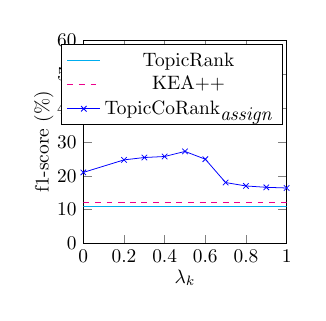
\begin{tikzpicture}[scale=.7]
                    \pgfkeys{/pgf/number format/.cd, fixed}
                    \begin{axis}[x=0.304152\linewidth,
                                 xtick={0, 0.2, 0.4, ..., 1},
                                 xmin=0,
                                 xmax=1,
                                 xlabel=$\lambda_k$,
                                 x label style={yshift=.34em},
                                 y=0.0050692\linewidth,
                                 ytick={0, 10, 20, ..., 100},
                                 ymin=0,
                                 ymax=60,
                                 ylabel=f1-score (\%),
                                 y label style={yshift=-.5em}]
                        \addplot[cyan] coordinates{
                            (0.0, 11)
                            (0.2, 11)
                            (0.3, 11)
                            (0.4, 11)
                            (0.5, 11)
                            (0.6, 11)
                            (0.7, 11)
                            (0.8, 11)
                            (0.9, 11)
                            (1.0, 11)
                        };
                        \addplot[magenta, dashed] coordinates{
                            (0.0, 12)
                            (0.2, 12)
                            (0.3, 12)
                            (0.4, 12)
                            (0.5, 12)
                            (0.6, 12)
                            (0.7, 12)
                            (0.8, 12)
                            (0.9, 12)
                            (1.0, 12)
                        };
                        \addplot[blue, mark=x] coordinates{
                            (0.0, 21.0)
                            (0.2, 24.7)
                            (0.3, 25.4)
                            (0.4, 25.7)
                            (0.5, 27.2)
                            (0.6, 24.9)
                            (0.7, 18.0)
                            (0.8, 17.0)
                            (0.9, 16.6)
                            (1.0, 16.4)
                        };
                        \legend{TopicRank, KEA++, TopicCoRank$_\textit{assign}$};
                    \end{axis}
                \end{tikzpicture}
            }
            \subfigure[Information Science]{
                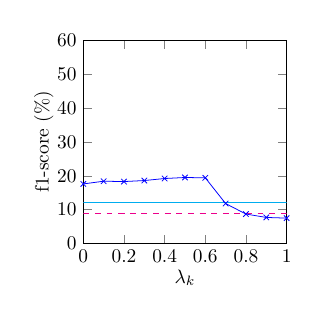
\begin{tikzpicture}[scale=.7]
                    \pgfkeys{/pgf/number format/.cd, fixed}
                    \begin{axis}[x=0.304152\linewidth,
                                 xtick={0, 0.2, 0.4, ..., 1},
                                 xmin=0,
                                 xmax=1,
                                 xlabel=$\lambda_k$,
                                 x label style={yshift=.34em},
                                 y=0.0050692\linewidth,
                                 ytick={0, 10, 20, ..., 100},
                                 ymin=0,
                                 ymax=60,
                                 ylabel=f1-score (\%),
                                 y label style={yshift=-.5em}]
                        \addplot[cyan] coordinates{
                            (0.0, 12)
                            (0.2, 12)
                            (0.3, 12)
                            (0.4, 12)
                            (0.5, 12)
                            (0.6, 12)
                            (0.7, 12)
                            (0.8, 12)
                            (0.9, 12)
                            (1.0, 12)
                        };
                        \addplot[magenta, dashed] coordinates{
                            (0.0, 9)
                            (0.2, 9)
                            (0.3, 9)
                            (0.4, 9)
                            (0.5, 9)
                            (0.6, 9)
                            (0.7, 9)
                            (0.8, 9)
                            (0.9, 9)
                            (1.0, 9)
                        };
                        \addplot[blue, mark=x] coordinates{
                            (0.0, 17.6)
                            (0.1, 18.4)
                            (0.2, 18.3)
                            (0.3, 18.6)
                            (0.4, 19.2)
                            (0.5, 19.5)
                            (0.6, 19.4)
                            (0.7, 11.8)
                            (0.8, 8.7)
                            (0.9, 7.7)
                            (1.0, 7.5)
                        };
                    \end{axis}
                \end{tikzpicture}
            }
            \subfigure[Archaeology]{
                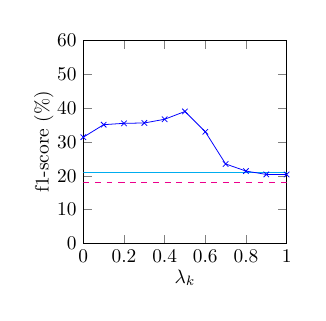
\begin{tikzpicture}[scale=.7]
                    \pgfkeys{/pgf/number format/.cd, fixed}
                    \begin{axis}[x=0.304152\linewidth,
                                 xtick={0, 0.2, 0.4, ..., 1},
                                 xmin=0,
                                 xmax=1,
                                 xlabel=$\lambda_k$,
                                 x label style={yshift=.34em},
                                 y=0.0050692\linewidth,
                                 ytick={0, 10, 20, ..., 100},
                                 ymin=0,
                                 ymax=60,
                                 ylabel=f1-score (\%),
                                 y label style={yshift=-.5em},
                                 legend style={font=\footnotesize}]
                        \addplot[cyan] coordinates{
                            (0.0, 21)
                            (0.2, 21)
                            (0.3, 21)
                            (0.4, 21)
                            (0.5, 21)
                            (0.6, 21)
                            (0.7, 21)
                            (0.8, 21)
                            (0.9, 21)
                            (1.0, 21)
                        };
                        \addplot[magenta, dashed] coordinates{
                            (0.0, 18)
                            (0.2, 18)
                            (0.3, 18)
                            (0.4, 18)
                            (0.5, 18)
                            (0.6, 18)
                            (0.7, 18)
                            (0.8, 18)
                            (0.9, 18)
                            (1.0, 18)
                        };
                        \addplot[blue, mark=x] coordinates{
                            (0.0, 31.4)
                            (0.1, 35.1)
                            (0.2, 35.5)
                            (0.3, 35.6)
                            (0.4, 36.7)
                            (0.5, 39.0)
                            (0.6, 33.0)
                            (0.7, 23.5)
                            (0.8, 21.4)
                            (0.9, 20.4)
                            (1.0, 20.4)
                        };
                    \end{axis}
                \end{tikzpicture}
            }
            \caption{
                Behavior of TopicCoRank$_\textit{assign}$ depending on $\lambda_k$ ($\lambda_t = 0.1$)
                \label{fig:lambda_k_variation}
            }
        \end{figure}
